% Copyright (c) 2022 by Lars Spreng
% This work is licensed under the Creative Commons Attribution 4.0 International License.
% To view a copy of this license, visit http://creativecommons.org/licenses/by/4.0/ or send a letter to Creative Commons, PO Box 1866, Mountain View, CA 94042, USA.
%
%~~~~~~~~~~~~~~~~~~~~~~~~~~~~~~~~~~~~~~~~~~~~~~~~~~~~~~~~~~~~~~~~~~~~~~~~~~~~~~
% Plan B: The Show Must Go On. Seven-minute hackathon presentation (420 s, 13 slides plus
% backup slides). Author: Noctis Zhang, University of Massachusetts Boston.
% Speaker notes for each slide live in the \note{...} blocks and match pres-note.md.
% Uncomment the \setbeameroption line below to see them.
%
% Every held-out number comes from figures/results_numbers.tex and figures/fig_results.tex, which
% ../make_results.py writes from the committed run wave3_heldout_20261025T1625Z (metrics.json),
% the evaluation of record of version 1.1. The version 1.2 numbers come from
% figures/results_numbers_v12.tex: fresh: is the held-out run wave3b_fresh_20261025T2327Z, and
% rerun: is wave3b_rerun_spent_20261025T2345Z, a post-hoc diagnostic rerun on spent cases.
%~~~~~~~~~~~~~~~~~~~~~~~~~~~~~~~~~~~~~~~~~~~~~~~~~~~~~~~~~~~~~~~~~~~~~~~~~~~~~~

\documentclass[
t,11pt,notheorems,usepdftitle=false,hyperref={pdfauthor={Noctis Zhang},pdftitle={Plan B: The Show Must Go On},pdfsubject={Seven-minute project presentation}}
]{beamer}
% Keep the PDF metadata to title, author and subject: no producer, creator or embedded file info.
\pdfsuppressptexinfo=-1
\hypersetup{pdfcreator={},pdfproducer={}}


% Copyright (c) 2022 by Lars Spreng
% This work is licensed under the Creative Commons Attribution 4.0 International License. 
% To view a copy of this license, visit http://creativecommons.org/licenses/by/4.0/ or send a letter to Creative Commons, PO Box 1866, Mountain View, CA 94042, USA.

%~~~~~~~~~~~~~~~~~~~~~~~~~~~~~~~~~~~~~~~~~~~~~~~~~~~~~~~~~~~~~~~~~~~~~~~~~~~~~~
% Add your packages and commands to this file
%~~~~~~~~~~~~~~~~~~~~~~~~~~~~~~~~~~~~~~~~~~~~~~~~~~~~~~~~~~~~~~~~~~~~~~~~~~~~~~

%~~~~~~~~~~~~~~~~~~~~~~~~~~~~~~~~~~~~~~~~~~~~~~~~~~~~~~~~~~~~~~~~~~~~~~~~~~~~~~
% Fonts
% \RequirePackage{palatino} % for serif slides
% \usefonttheme{serif}
\RequirePackage[scaled]{helvet} % for sans-serif slides

\RequirePackage[utf8]{inputenc}
\RequirePackage[T1]{fontenc}


\usepackage{styles/elegantmacros}
\usefolder{styles}
\usetheme[style=gray]{elegant}

\newcommand{\makepart}[1]{ % For convenience
\part{#1} \frame{\partpage}
}

%~~~~~~~~~~~~~~~~~~~~~~~~~~~~~~~~~~~~~~~~~~~~~~~~~~~~~~~~~~~~~~~~~~~~~~~~~~~~~~

%~~~~~~~~~~~~~~~~~~~~~~~~~~~~~~~~~~~~~~~~~~~~~~~~~~~~~~~~~~~~~~~~~~~~~~~~~~~~~~
% Figures
\RequirePackage{booktabs}
\RequirePackage{colortbl}
\RequirePackage{ragged2e}
\RequirePackage{schemabloc}
%\RequirePackage{natbib}
\RequirePackage{caption}
\RequirePackage{subcaption}
\RequirePackage{tabularx}
\RequirePackage{array}
\RequirePackage{multirow}
% biblatex and references.bib from the template are not used by this deck.
\newcolumntype{Y}{>{\centering\arraybackslash}X}

%~~~~~~~~~~~~~~~~~~~~~~~~~~~~~~~~~~~~~~~~~~~~~~~~~~~~~~~~~~~~~~~~~~~~~~~~~~~~~~

%~~~~~~~~~~~~~~~~~~~~~~~~~~~~~~~~~~~~~~~~~~~~~~~~~~~~~~~~~~~~~~~~~~~~~~~~~~~~~~
% Figures
\RequirePackage{wrapfig}
\RequirePackage{pgfplots}
\RequirePackage{graphicx}
\RequirePackage{adjustbox}
\RequirePackage{environ}
\pgfplotsset{compat=1.18}

\makeatletter
\newsavebox{\measure@tikzpicture}
\NewEnviron{scaletikzpicturetowidth}[1]{%
  \def\tikz@width{#1}%
  \def\tikzscale{1}\begin{lrbox}{\measure@tikzpicture}%
  \BODY
  \end{lrbox}%
  \pgfmathparse{#1/\wd\measure@tikzpicture}%
  \edef\tikzscale{\pgfmathresult}%
  \BODY
}
\makeatother
%~~~~~~~~~~~~~~~~~~~~~~~~~~~~~~~~~~~~~~~~~~~~~~~~~~~~~~~~~~~~~~~~~~~~~~~~~~~~~~

%~~~~~~~~~~~~~~~~~~~~~~~~~~~~~~~~~~~~~~~~~~~~~~~~~~~~~~~~~~~~~~~~~~~~~~~~~~~~~~
% Maths 
\RequirePackage{textcomp}
\RequirePackage{amsmath} 
\RequirePackage{amsthm}
\RequirePackage{mathtools}
%\RequirePackage{bbm}
%\RequirePackage{algorithm}
%\RequirePackage[osf,sc]{mathpazo}
%\RequirePackage{pifont}
%\newcommand{\xmark}{\ding{55}}%
%\numberwithin{equation}{section}
\DeclareMathOperator*{\argmax}{arg\,max}
\DeclareMathOperator*{\argmin}{arg\,min}

\setbeamertemplate{theorems}[numbered] % to number

\theoremstyle{definition}
\newtheorem{fact}{Fact}[section]
\newtheorem{examp}{Example}[section]

\theoremstyle{plain}
\newtheorem{definition}{Definition}[section]
\newtheorem{proposition}{Proposition}
\newtheorem{theorem}{Theorem}
\newtheorem{assumption}{Assumption}

\providecommand{\H}{\mathscr{H}}      
\providecommand{\E}{\mathbb{E}}
\makeatletter
\def\munderbar#1{\underline{\sbox\tw@{$#1$}\dp\tw@\z@\box\tw@}}
\makeatother

%~~~~~~~~~~~~~~~~~~~~~~~~~~~~~~~~~~~~~~~~~~~~~~~~~~~~~~~~~~~~~~~~~~~~~~~~~~~~~~
 % Loads packages and some defined commands
\usepackage{appendixnumberbeamer} % backups are not counted in the slide total
% Written by make_results.py from wave3_heldout_20261025T1625Z/<suite>/report/metrics.json. Do not edit.
\providecommand{\res}[1]{\csname res:#1\endcsname}
\expandafter\def\csname res:campus:P0:goal\endcsname{5/7}
\expandafter\def\csname res:campus:P0:infeas\endcsname{1/1}
\expandafter\def\csname res:campus:P0:met\endcsname{6/8}
\expandafter\def\csname res:campus:P0:metk\endcsname{6}
\expandafter\def\csname res:campus:P0:metn\endcsname{8}
\expandafter\def\csname res:campus:P0:cases\endcsname{6}
\expandafter\def\csname res:campus:P0:ncases\endcsname{8}
\expandafter\def\csname res:campus:P0:recorded\endcsname{8}
\expandafter\def\csname res:campus:P0:planned\endcsname{8}
\expandafter\def\csname res:campus:P0:capped\endcsname{0}
\expandafter\def\csname res:campus:P0:viol\endcsname{0}
\expandafter\def\csname res:campus:P0:refused\endcsname{0}
\expandafter\def\csname res:campus:P0:unnec\endcsname{0}
\expandafter\def\csname res:campus:P0:unnecn\endcsname{3}
\expandafter\def\csname res:campus:P0:usd\endcsname{0.00}
\expandafter\def\csname res:campus:P0:calls\endcsname{0}
\expandafter\def\csname res:campus:P0:checks\endcsname{0.9}
\expandafter\def\csname res:campus:P1:goal\endcsname{21/21}
\expandafter\def\csname res:campus:P1:infeas\endcsname{3/3}
\expandafter\def\csname res:campus:P1:met\endcsname{24/24}
\expandafter\def\csname res:campus:P1:metk\endcsname{24}
\expandafter\def\csname res:campus:P1:metn\endcsname{24}
\expandafter\def\csname res:campus:P1:cases\endcsname{8}
\expandafter\def\csname res:campus:P1:ncases\endcsname{8}
\expandafter\def\csname res:campus:P1:recorded\endcsname{24}
\expandafter\def\csname res:campus:P1:planned\endcsname{24}
\expandafter\def\csname res:campus:P1:capped\endcsname{0}
\expandafter\def\csname res:campus:P1:viol\endcsname{0}
\expandafter\def\csname res:campus:P1:refused\endcsname{5}
\expandafter\def\csname res:campus:P1:unnec\endcsname{0}
\expandafter\def\csname res:campus:P1:unnecn\endcsname{9}
\expandafter\def\csname res:campus:P1:usd\endcsname{3.01}
\expandafter\def\csname res:campus:P1:calls\endcsname{90}
\expandafter\def\csname res:campus:P1:checks\endcsname{2.0}
\expandafter\def\csname res:campus:P2:goal\endcsname{15/21}
\expandafter\def\csname res:campus:P2:infeas\endcsname{3/3}
\expandafter\def\csname res:campus:P2:met\endcsname{18/24}
\expandafter\def\csname res:campus:P2:metk\endcsname{18}
\expandafter\def\csname res:campus:P2:metn\endcsname{24}
\expandafter\def\csname res:campus:P2:cases\endcsname{6}
\expandafter\def\csname res:campus:P2:ncases\endcsname{8}
\expandafter\def\csname res:campus:P2:recorded\endcsname{24}
\expandafter\def\csname res:campus:P2:planned\endcsname{24}
\expandafter\def\csname res:campus:P2:capped\endcsname{3}
\expandafter\def\csname res:campus:P2:viol\endcsname{0}
\expandafter\def\csname res:campus:P2:refused\endcsname{0}
\expandafter\def\csname res:campus:P2:unnec\endcsname{0}
\expandafter\def\csname res:campus:P2:unnecn\endcsname{9}
\expandafter\def\csname res:campus:P2:usd\endcsname{1.00}
\expandafter\def\csname res:campus:P2:calls\endcsname{84}
\expandafter\def\csname res:campus:P2:checks\endcsname{1.3}
\expandafter\def\csname res:campus:P3:goal\endcsname{18/21}
\expandafter\def\csname res:campus:P3:infeas\endcsname{3/3}
\expandafter\def\csname res:campus:P3:met\endcsname{21/24}
\expandafter\def\csname res:campus:P3:metk\endcsname{21}
\expandafter\def\csname res:campus:P3:metn\endcsname{24}
\expandafter\def\csname res:campus:P3:cases\endcsname{7}
\expandafter\def\csname res:campus:P3:ncases\endcsname{8}
\expandafter\def\csname res:campus:P3:recorded\endcsname{24}
\expandafter\def\csname res:campus:P3:planned\endcsname{24}
\expandafter\def\csname res:campus:P3:capped\endcsname{0}
\expandafter\def\csname res:campus:P3:viol\endcsname{0}
\expandafter\def\csname res:campus:P3:refused\endcsname{6}
\expandafter\def\csname res:campus:P3:unnec\endcsname{0}
\expandafter\def\csname res:campus:P3:unnecn\endcsname{9}
\expandafter\def\csname res:campus:P3:usd\endcsname{0.57}
\expandafter\def\csname res:campus:P3:calls\endcsname{57}
\expandafter\def\csname res:campus:P3:checks\endcsname{2.1}
\expandafter\def\csname res:campus:all:recorded\endcsname{80}
\expandafter\def\csname res:campus:all:planned\endcsname{80}
\expandafter\def\csname res:campus:all:viol\endcsname{0}
\expandafter\def\csname res:campus:all:refused\endcsname{11}
\expandafter\def\csname res:campus:all:unnec\endcsname{0}
\expandafter\def\csname res:campus:all:stale\endcsname{11}
\expandafter\def\csname res:campus:all:capped\endcsname{3}
\expandafter\def\csname res:campus:all:missing\endcsname{0}
\expandafter\def\csname res:campus:all:aborted\endcsname{0}
\expandafter\def\csname res:pantry:P0:target\endcsname{2/2}
\expandafter\def\csname res:pantry:P0:partial\endcsname{2/2}
\expandafter\def\csname res:pantry:P0:met\endcsname{4/4}
\expandafter\def\csname res:pantry:P0:metk\endcsname{4}
\expandafter\def\csname res:pantry:P0:metn\endcsname{4}
\expandafter\def\csname res:pantry:P0:cases\endcsname{4}
\expandafter\def\csname res:pantry:P0:ncases\endcsname{4}
\expandafter\def\csname res:pantry:P0:recorded\endcsname{4}
\expandafter\def\csname res:pantry:P0:planned\endcsname{4}
\expandafter\def\csname res:pantry:P0:capped\endcsname{0}
\expandafter\def\csname res:pantry:P0:viol\endcsname{0}
\expandafter\def\csname res:pantry:P0:refused\endcsname{5}
\expandafter\def\csname res:pantry:P0:unnec\endcsname{0}
\expandafter\def\csname res:pantry:P0:unnecn\endcsname{0}
\expandafter\def\csname res:pantry:P0:usd\endcsname{0.00}
\expandafter\def\csname res:pantry:P0:calls\endcsname{0}
\expandafter\def\csname res:pantry:P0:checks\endcsname{2.0}
\expandafter\def\csname res:pantry:P0:kits\endcsname{138/160}
\expandafter\def\csname res:pantry:P0:conserv\endcsname{0}
\expandafter\def\csname res:pantry:P0:credits\endcsname{0}
\expandafter\def\csname res:pantry:P1:target\endcsname{6/6}
\expandafter\def\csname res:pantry:P1:partial\endcsname{0/6}
\expandafter\def\csname res:pantry:P1:met\endcsname{6/12}
\expandafter\def\csname res:pantry:P1:metk\endcsname{6}
\expandafter\def\csname res:pantry:P1:metn\endcsname{12}
\expandafter\def\csname res:pantry:P1:cases\endcsname{2}
\expandafter\def\csname res:pantry:P1:ncases\endcsname{4}
\expandafter\def\csname res:pantry:P1:recorded\endcsname{12}
\expandafter\def\csname res:pantry:P1:planned\endcsname{12}
\expandafter\def\csname res:pantry:P1:capped\endcsname{6}
\expandafter\def\csname res:pantry:P1:viol\endcsname{0}
\expandafter\def\csname res:pantry:P1:refused\endcsname{12}
\expandafter\def\csname res:pantry:P1:unnec\endcsname{0}
\expandafter\def\csname res:pantry:P1:unnecn\endcsname{0}
\expandafter\def\csname res:pantry:P1:usd\endcsname{2.56}
\expandafter\def\csname res:pantry:P1:calls\endcsname{84}
\expandafter\def\csname res:pantry:P1:checks\endcsname{1.4}
\expandafter\def\csname res:pantry:P1:kits\endcsname{240/480}
\expandafter\def\csname res:pantry:P1:conserv\endcsname{0}
\expandafter\def\csname res:pantry:P1:credits\endcsname{0}
\expandafter\def\csname res:pantry:P2:target\endcsname{6/6}
\expandafter\def\csname res:pantry:P2:partial\endcsname{3/6}
\expandafter\def\csname res:pantry:P2:met\endcsname{9/12}
\expandafter\def\csname res:pantry:P2:metk\endcsname{9}
\expandafter\def\csname res:pantry:P2:metn\endcsname{12}
\expandafter\def\csname res:pantry:P2:cases\endcsname{3}
\expandafter\def\csname res:pantry:P2:ncases\endcsname{4}
\expandafter\def\csname res:pantry:P2:recorded\endcsname{12}
\expandafter\def\csname res:pantry:P2:planned\endcsname{12}
\expandafter\def\csname res:pantry:P2:capped\endcsname{6}
\expandafter\def\csname res:pantry:P2:viol\endcsname{0}
\expandafter\def\csname res:pantry:P2:refused\endcsname{9}
\expandafter\def\csname res:pantry:P2:unnec\endcsname{0}
\expandafter\def\csname res:pantry:P2:unnecn\endcsname{0}
\expandafter\def\csname res:pantry:P2:usd\endcsname{0.95}
\expandafter\def\csname res:pantry:P2:calls\endcsname{83}
\expandafter\def\csname res:pantry:P2:checks\endcsname{0.7}
\expandafter\def\csname res:pantry:P2:kits\endcsname{342/480}
\expandafter\def\csname res:pantry:P2:conserv\endcsname{0}
\expandafter\def\csname res:pantry:P2:credits\endcsname{0}
\expandafter\def\csname res:pantry:P3:target\endcsname{3/6}
\expandafter\def\csname res:pantry:P3:partial\endcsname{3/6}
\expandafter\def\csname res:pantry:P3:met\endcsname{6/12}
\expandafter\def\csname res:pantry:P3:metk\endcsname{6}
\expandafter\def\csname res:pantry:P3:metn\endcsname{12}
\expandafter\def\csname res:pantry:P3:cases\endcsname{2}
\expandafter\def\csname res:pantry:P3:ncases\endcsname{4}
\expandafter\def\csname res:pantry:P3:recorded\endcsname{12}
\expandafter\def\csname res:pantry:P3:planned\endcsname{12}
\expandafter\def\csname res:pantry:P3:capped\endcsname{6}
\expandafter\def\csname res:pantry:P3:viol\endcsname{0}
\expandafter\def\csname res:pantry:P3:refused\endcsname{18}
\expandafter\def\csname res:pantry:P3:unnec\endcsname{0}
\expandafter\def\csname res:pantry:P3:unnecn\endcsname{0}
\expandafter\def\csname res:pantry:P3:usd\endcsname{0.99}
\expandafter\def\csname res:pantry:P3:calls\endcsname{84}
\expandafter\def\csname res:pantry:P3:checks\endcsname{3.2}
\expandafter\def\csname res:pantry:P3:kits\endcsname{294/480}
\expandafter\def\csname res:pantry:P3:conserv\endcsname{0}
\expandafter\def\csname res:pantry:P3:credits\endcsname{0}
\expandafter\def\csname res:pantry:all:recorded\endcsname{40}
\expandafter\def\csname res:pantry:all:planned\endcsname{40}
\expandafter\def\csname res:pantry:all:viol\endcsname{0}
\expandafter\def\csname res:pantry:all:refused\endcsname{44}
\expandafter\def\csname res:pantry:all:unnec\endcsname{0}
\expandafter\def\csname res:pantry:all:stale\endcsname{28}
\expandafter\def\csname res:pantry:all:capped\endcsname{18}
\expandafter\def\csname res:pantry:all:missing\endcsname{0}
\expandafter\def\csname res:pantry:all:aborted\endcsname{0}
\expandafter\def\csname res:both:recorded\endcsname{120}
\expandafter\def\csname res:both:planned\endcsname{120}
\expandafter\def\csname res:both:viol\endcsname{0}
\expandafter\def\csname res:both:refused\endcsname{55}
\expandafter\def\csname res:both:stale\endcsname{39}
\expandafter\def\csname res:both:unnec\endcsname{0}
\expandafter\def\csname res:both:capped\endcsname{21}
 % Held-out numbers, read as \res{suite:policy:key}
% Written by make_results.py from wave3b_fresh_20261025T2327Z (fresh), wave3b_rerun_spent_20261025T2345Z (rerun), <suite>/report/metrics.json. Do not edit.
\providecommand{\res}[1]{\csname res:#1\endcsname}
\expandafter\def\csname res:fresh:campus:P0:goal\endcsname{2/3}
\expandafter\def\csname res:fresh:campus:P0:infeas\endcsname{1/1}
\expandafter\def\csname res:fresh:campus:P0:met\endcsname{3/4}
\expandafter\def\csname res:fresh:campus:P0:metk\endcsname{3}
\expandafter\def\csname res:fresh:campus:P0:metn\endcsname{4}
\expandafter\def\csname res:fresh:campus:P0:cases\endcsname{3}
\expandafter\def\csname res:fresh:campus:P0:ncases\endcsname{4}
\expandafter\def\csname res:fresh:campus:P0:recorded\endcsname{4}
\expandafter\def\csname res:fresh:campus:P0:planned\endcsname{4}
\expandafter\def\csname res:fresh:campus:P0:capped\endcsname{0}
\expandafter\def\csname res:fresh:campus:P0:viol\endcsname{0}
\expandafter\def\csname res:fresh:campus:P0:refused\endcsname{0}
\expandafter\def\csname res:fresh:campus:P0:unnec\endcsname{0}
\expandafter\def\csname res:fresh:campus:P0:unnecn\endcsname{1}
\expandafter\def\csname res:fresh:campus:P0:usd\endcsname{0.00}
\expandafter\def\csname res:fresh:campus:P0:calls\endcsname{0}
\expandafter\def\csname res:fresh:campus:P0:checks\endcsname{1.0}
\expandafter\def\csname res:fresh:campus:P1:goal\endcsname{9/9}
\expandafter\def\csname res:fresh:campus:P1:infeas\endcsname{3/3}
\expandafter\def\csname res:fresh:campus:P1:met\endcsname{12/12}
\expandafter\def\csname res:fresh:campus:P1:metk\endcsname{12}
\expandafter\def\csname res:fresh:campus:P1:metn\endcsname{12}
\expandafter\def\csname res:fresh:campus:P1:cases\endcsname{4}
\expandafter\def\csname res:fresh:campus:P1:ncases\endcsname{4}
\expandafter\def\csname res:fresh:campus:P1:recorded\endcsname{12}
\expandafter\def\csname res:fresh:campus:P1:planned\endcsname{12}
\expandafter\def\csname res:fresh:campus:P1:capped\endcsname{0}
\expandafter\def\csname res:fresh:campus:P1:viol\endcsname{0}
\expandafter\def\csname res:fresh:campus:P1:refused\endcsname{0}
\expandafter\def\csname res:fresh:campus:P1:unnec\endcsname{0}
\expandafter\def\csname res:fresh:campus:P1:unnecn\endcsname{3}
\expandafter\def\csname res:fresh:campus:P1:usd\endcsname{1.17}
\expandafter\def\csname res:fresh:campus:P1:calls\endcsname{36}
\expandafter\def\csname res:fresh:campus:P1:checks\endcsname{1.2}
\expandafter\def\csname res:fresh:campus:P2:goal\endcsname{9/9}
\expandafter\def\csname res:fresh:campus:P2:infeas\endcsname{3/3}
\expandafter\def\csname res:fresh:campus:P2:met\endcsname{12/12}
\expandafter\def\csname res:fresh:campus:P2:metk\endcsname{12}
\expandafter\def\csname res:fresh:campus:P2:metn\endcsname{12}
\expandafter\def\csname res:fresh:campus:P2:cases\endcsname{4}
\expandafter\def\csname res:fresh:campus:P2:ncases\endcsname{4}
\expandafter\def\csname res:fresh:campus:P2:recorded\endcsname{12}
\expandafter\def\csname res:fresh:campus:P2:planned\endcsname{12}
\expandafter\def\csname res:fresh:campus:P2:capped\endcsname{0}
\expandafter\def\csname res:fresh:campus:P2:viol\endcsname{0}
\expandafter\def\csname res:fresh:campus:P2:refused\endcsname{0}
\expandafter\def\csname res:fresh:campus:P2:unnec\endcsname{0}
\expandafter\def\csname res:fresh:campus:P2:unnecn\endcsname{3}
\expandafter\def\csname res:fresh:campus:P2:usd\endcsname{0.34}
\expandafter\def\csname res:fresh:campus:P2:calls\endcsname{30}
\expandafter\def\csname res:fresh:campus:P2:checks\endcsname{0.8}
\expandafter\def\csname res:fresh:campus:P3:goal\endcsname{9/9}
\expandafter\def\csname res:fresh:campus:P3:infeas\endcsname{3/3}
\expandafter\def\csname res:fresh:campus:P3:met\endcsname{12/12}
\expandafter\def\csname res:fresh:campus:P3:metk\endcsname{12}
\expandafter\def\csname res:fresh:campus:P3:metn\endcsname{12}
\expandafter\def\csname res:fresh:campus:P3:cases\endcsname{4}
\expandafter\def\csname res:fresh:campus:P3:ncases\endcsname{4}
\expandafter\def\csname res:fresh:campus:P3:recorded\endcsname{12}
\expandafter\def\csname res:fresh:campus:P3:planned\endcsname{12}
\expandafter\def\csname res:fresh:campus:P3:capped\endcsname{0}
\expandafter\def\csname res:fresh:campus:P3:viol\endcsname{0}
\expandafter\def\csname res:fresh:campus:P3:refused\endcsname{0}
\expandafter\def\csname res:fresh:campus:P3:unnec\endcsname{0}
\expandafter\def\csname res:fresh:campus:P3:unnecn\endcsname{3}
\expandafter\def\csname res:fresh:campus:P3:usd\endcsname{0.21}
\expandafter\def\csname res:fresh:campus:P3:calls\endcsname{21}
\expandafter\def\csname res:fresh:campus:P3:checks\endcsname{1.5}
\expandafter\def\csname res:fresh:campus:all:recorded\endcsname{40}
\expandafter\def\csname res:fresh:campus:all:planned\endcsname{40}
\expandafter\def\csname res:fresh:campus:all:viol\endcsname{0}
\expandafter\def\csname res:fresh:campus:all:refused\endcsname{0}
\expandafter\def\csname res:fresh:campus:all:unnec\endcsname{0}
\expandafter\def\csname res:fresh:campus:all:stale\endcsname{0}
\expandafter\def\csname res:fresh:campus:all:capped\endcsname{0}
\expandafter\def\csname res:fresh:campus:all:missing\endcsname{0}
\expandafter\def\csname res:fresh:campus:all:aborted\endcsname{0}
\expandafter\def\csname res:fresh:pantry:P0:target\endcsname{1/1}
\expandafter\def\csname res:fresh:pantry:P0:partial\endcsname{1/1}
\expandafter\def\csname res:fresh:pantry:P0:met\endcsname{2/2}
\expandafter\def\csname res:fresh:pantry:P0:metk\endcsname{2}
\expandafter\def\csname res:fresh:pantry:P0:metn\endcsname{2}
\expandafter\def\csname res:fresh:pantry:P0:cases\endcsname{2}
\expandafter\def\csname res:fresh:pantry:P0:ncases\endcsname{2}
\expandafter\def\csname res:fresh:pantry:P0:recorded\endcsname{2}
\expandafter\def\csname res:fresh:pantry:P0:planned\endcsname{2}
\expandafter\def\csname res:fresh:pantry:P0:capped\endcsname{0}
\expandafter\def\csname res:fresh:pantry:P0:viol\endcsname{0}
\expandafter\def\csname res:fresh:pantry:P0:refused\endcsname{1}
\expandafter\def\csname res:fresh:pantry:P0:unnec\endcsname{0}
\expandafter\def\csname res:fresh:pantry:P0:unnecn\endcsname{0}
\expandafter\def\csname res:fresh:pantry:P0:usd\endcsname{0.00}
\expandafter\def\csname res:fresh:pantry:P0:calls\endcsname{0}
\expandafter\def\csname res:fresh:pantry:P0:checks\endcsname{2.0}
\expandafter\def\csname res:fresh:pantry:P0:kits\endcsname{64/80}
\expandafter\def\csname res:fresh:pantry:P0:conserv\endcsname{0}
\expandafter\def\csname res:fresh:pantry:P0:credits\endcsname{0}
\expandafter\def\csname res:fresh:pantry:P1:target\endcsname{3/3}
\expandafter\def\csname res:fresh:pantry:P1:partial\endcsname{3/3}
\expandafter\def\csname res:fresh:pantry:P1:met\endcsname{6/6}
\expandafter\def\csname res:fresh:pantry:P1:metk\endcsname{6}
\expandafter\def\csname res:fresh:pantry:P1:metn\endcsname{6}
\expandafter\def\csname res:fresh:pantry:P1:cases\endcsname{2}
\expandafter\def\csname res:fresh:pantry:P1:ncases\endcsname{2}
\expandafter\def\csname res:fresh:pantry:P1:recorded\endcsname{6}
\expandafter\def\csname res:fresh:pantry:P1:planned\endcsname{6}
\expandafter\def\csname res:fresh:pantry:P1:capped\endcsname{0}
\expandafter\def\csname res:fresh:pantry:P1:viol\endcsname{0}
\expandafter\def\csname res:fresh:pantry:P1:refused\endcsname{2}
\expandafter\def\csname res:fresh:pantry:P1:unnec\endcsname{0}
\expandafter\def\csname res:fresh:pantry:P1:unnecn\endcsname{0}
\expandafter\def\csname res:fresh:pantry:P1:usd\endcsname{1.15}
\expandafter\def\csname res:fresh:pantry:P1:calls\endcsname{38}
\expandafter\def\csname res:fresh:pantry:P1:checks\endcsname{1.7}
\expandafter\def\csname res:fresh:pantry:P1:kits\endcsname{192/240}
\expandafter\def\csname res:fresh:pantry:P1:conserv\endcsname{0}
\expandafter\def\csname res:fresh:pantry:P1:credits\endcsname{0}
\expandafter\def\csname res:fresh:pantry:P2:target\endcsname{3/3}
\expandafter\def\csname res:fresh:pantry:P2:partial\endcsname{3/3}
\expandafter\def\csname res:fresh:pantry:P2:met\endcsname{6/6}
\expandafter\def\csname res:fresh:pantry:P2:metk\endcsname{6}
\expandafter\def\csname res:fresh:pantry:P2:metn\endcsname{6}
\expandafter\def\csname res:fresh:pantry:P2:cases\endcsname{2}
\expandafter\def\csname res:fresh:pantry:P2:ncases\endcsname{2}
\expandafter\def\csname res:fresh:pantry:P2:recorded\endcsname{6}
\expandafter\def\csname res:fresh:pantry:P2:planned\endcsname{6}
\expandafter\def\csname res:fresh:pantry:P2:capped\endcsname{0}
\expandafter\def\csname res:fresh:pantry:P2:viol\endcsname{0}
\expandafter\def\csname res:fresh:pantry:P2:refused\endcsname{3}
\expandafter\def\csname res:fresh:pantry:P2:unnec\endcsname{0}
\expandafter\def\csname res:fresh:pantry:P2:unnecn\endcsname{0}
\expandafter\def\csname res:fresh:pantry:P2:usd\endcsname{0.42}
\expandafter\def\csname res:fresh:pantry:P2:calls\endcsname{39}
\expandafter\def\csname res:fresh:pantry:P2:checks\endcsname{1.0}
\expandafter\def\csname res:fresh:pantry:P2:kits\endcsname{192/240}
\expandafter\def\csname res:fresh:pantry:P2:conserv\endcsname{0}
\expandafter\def\csname res:fresh:pantry:P2:credits\endcsname{0}
\expandafter\def\csname res:fresh:pantry:P3:target\endcsname{3/3}
\expandafter\def\csname res:fresh:pantry:P3:partial\endcsname{3/3}
\expandafter\def\csname res:fresh:pantry:P3:met\endcsname{6/6}
\expandafter\def\csname res:fresh:pantry:P3:metk\endcsname{6}
\expandafter\def\csname res:fresh:pantry:P3:metn\endcsname{6}
\expandafter\def\csname res:fresh:pantry:P3:cases\endcsname{2}
\expandafter\def\csname res:fresh:pantry:P3:ncases\endcsname{2}
\expandafter\def\csname res:fresh:pantry:P3:recorded\endcsname{6}
\expandafter\def\csname res:fresh:pantry:P3:planned\endcsname{6}
\expandafter\def\csname res:fresh:pantry:P3:capped\endcsname{0}
\expandafter\def\csname res:fresh:pantry:P3:viol\endcsname{0}
\expandafter\def\csname res:fresh:pantry:P3:refused\endcsname{0}
\expandafter\def\csname res:fresh:pantry:P3:unnec\endcsname{0}
\expandafter\def\csname res:fresh:pantry:P3:unnecn\endcsname{0}
\expandafter\def\csname res:fresh:pantry:P3:usd\endcsname{0.32}
\expandafter\def\csname res:fresh:pantry:P3:calls\endcsname{30}
\expandafter\def\csname res:fresh:pantry:P3:checks\endcsname{2.5}
\expandafter\def\csname res:fresh:pantry:P3:kits\endcsname{192/240}
\expandafter\def\csname res:fresh:pantry:P3:conserv\endcsname{0}
\expandafter\def\csname res:fresh:pantry:P3:credits\endcsname{0}
\expandafter\def\csname res:fresh:pantry:all:recorded\endcsname{20}
\expandafter\def\csname res:fresh:pantry:all:planned\endcsname{20}
\expandafter\def\csname res:fresh:pantry:all:viol\endcsname{0}
\expandafter\def\csname res:fresh:pantry:all:refused\endcsname{6}
\expandafter\def\csname res:fresh:pantry:all:unnec\endcsname{0}
\expandafter\def\csname res:fresh:pantry:all:stale\endcsname{1}
\expandafter\def\csname res:fresh:pantry:all:capped\endcsname{0}
\expandafter\def\csname res:fresh:pantry:all:missing\endcsname{0}
\expandafter\def\csname res:fresh:pantry:all:aborted\endcsname{0}
\expandafter\def\csname res:fresh:both:recorded\endcsname{60}
\expandafter\def\csname res:fresh:both:planned\endcsname{60}
\expandafter\def\csname res:fresh:both:viol\endcsname{0}
\expandafter\def\csname res:fresh:both:refused\endcsname{6}
\expandafter\def\csname res:fresh:both:stale\endcsname{1}
\expandafter\def\csname res:fresh:both:unnec\endcsname{0}
\expandafter\def\csname res:fresh:both:capped\endcsname{0}
\expandafter\def\csname res:fresh:both:usd\endcsname{3.61}
\expandafter\def\csname res:fresh:both:metk\endcsname{59}
\expandafter\def\csname res:fresh:both:metn\endcsname{60}
\expandafter\def\csname res:rerun:campus:P0:goal\endcsname{5/7}
\expandafter\def\csname res:rerun:campus:P0:infeas\endcsname{1/1}
\expandafter\def\csname res:rerun:campus:P0:met\endcsname{6/8}
\expandafter\def\csname res:rerun:campus:P0:metk\endcsname{6}
\expandafter\def\csname res:rerun:campus:P0:metn\endcsname{8}
\expandafter\def\csname res:rerun:campus:P0:cases\endcsname{6}
\expandafter\def\csname res:rerun:campus:P0:ncases\endcsname{8}
\expandafter\def\csname res:rerun:campus:P0:recorded\endcsname{8}
\expandafter\def\csname res:rerun:campus:P0:planned\endcsname{8}
\expandafter\def\csname res:rerun:campus:P0:capped\endcsname{0}
\expandafter\def\csname res:rerun:campus:P0:viol\endcsname{0}
\expandafter\def\csname res:rerun:campus:P0:refused\endcsname{0}
\expandafter\def\csname res:rerun:campus:P0:unnec\endcsname{0}
\expandafter\def\csname res:rerun:campus:P0:unnecn\endcsname{3}
\expandafter\def\csname res:rerun:campus:P0:usd\endcsname{0.00}
\expandafter\def\csname res:rerun:campus:P0:calls\endcsname{0}
\expandafter\def\csname res:rerun:campus:P0:checks\endcsname{0.9}
\expandafter\def\csname res:rerun:campus:P1:goal\endcsname{21/21}
\expandafter\def\csname res:rerun:campus:P1:infeas\endcsname{3/3}
\expandafter\def\csname res:rerun:campus:P1:met\endcsname{24/24}
\expandafter\def\csname res:rerun:campus:P1:metk\endcsname{24}
\expandafter\def\csname res:rerun:campus:P1:metn\endcsname{24}
\expandafter\def\csname res:rerun:campus:P1:cases\endcsname{8}
\expandafter\def\csname res:rerun:campus:P1:ncases\endcsname{8}
\expandafter\def\csname res:rerun:campus:P1:recorded\endcsname{24}
\expandafter\def\csname res:rerun:campus:P1:planned\endcsname{24}
\expandafter\def\csname res:rerun:campus:P1:capped\endcsname{1}
\expandafter\def\csname res:rerun:campus:P1:viol\endcsname{0}
\expandafter\def\csname res:rerun:campus:P1:refused\endcsname{3}
\expandafter\def\csname res:rerun:campus:P1:unnec\endcsname{0}
\expandafter\def\csname res:rerun:campus:P1:unnecn\endcsname{9}
\expandafter\def\csname res:rerun:campus:P1:usd\endcsname{3.00}
\expandafter\def\csname res:rerun:campus:P1:calls\endcsname{90}
\expandafter\def\csname res:rerun:campus:P1:checks\endcsname{1.8}
\expandafter\def\csname res:rerun:campus:P2:goal\endcsname{18/21}
\expandafter\def\csname res:rerun:campus:P2:infeas\endcsname{3/3}
\expandafter\def\csname res:rerun:campus:P2:met\endcsname{21/24}
\expandafter\def\csname res:rerun:campus:P2:metk\endcsname{21}
\expandafter\def\csname res:rerun:campus:P2:metn\endcsname{24}
\expandafter\def\csname res:rerun:campus:P2:cases\endcsname{7}
\expandafter\def\csname res:rerun:campus:P2:ncases\endcsname{8}
\expandafter\def\csname res:rerun:campus:P2:recorded\endcsname{24}
\expandafter\def\csname res:rerun:campus:P2:planned\endcsname{24}
\expandafter\def\csname res:rerun:campus:P2:capped\endcsname{3}
\expandafter\def\csname res:rerun:campus:P2:viol\endcsname{0}
\expandafter\def\csname res:rerun:campus:P2:refused\endcsname{0}
\expandafter\def\csname res:rerun:campus:P2:unnec\endcsname{0}
\expandafter\def\csname res:rerun:campus:P2:unnecn\endcsname{9}
\expandafter\def\csname res:rerun:campus:P2:usd\endcsname{1.04}
\expandafter\def\csname res:rerun:campus:P2:calls\endcsname{87}
\expandafter\def\csname res:rerun:campus:P2:checks\endcsname{1.3}
\expandafter\def\csname res:rerun:campus:P3:goal\endcsname{21/21}
\expandafter\def\csname res:rerun:campus:P3:infeas\endcsname{3/3}
\expandafter\def\csname res:rerun:campus:P3:met\endcsname{24/24}
\expandafter\def\csname res:rerun:campus:P3:metk\endcsname{24}
\expandafter\def\csname res:rerun:campus:P3:metn\endcsname{24}
\expandafter\def\csname res:rerun:campus:P3:cases\endcsname{8}
\expandafter\def\csname res:rerun:campus:P3:ncases\endcsname{8}
\expandafter\def\csname res:rerun:campus:P3:recorded\endcsname{24}
\expandafter\def\csname res:rerun:campus:P3:planned\endcsname{24}
\expandafter\def\csname res:rerun:campus:P3:capped\endcsname{0}
\expandafter\def\csname res:rerun:campus:P3:viol\endcsname{0}
\expandafter\def\csname res:rerun:campus:P3:refused\endcsname{6}
\expandafter\def\csname res:rerun:campus:P3:unnec\endcsname{0}
\expandafter\def\csname res:rerun:campus:P3:unnecn\endcsname{9}
\expandafter\def\csname res:rerun:campus:P3:usd\endcsname{0.53}
\expandafter\def\csname res:rerun:campus:P3:calls\endcsname{54}
\expandafter\def\csname res:rerun:campus:P3:checks\endcsname{2.1}
\expandafter\def\csname res:rerun:campus:all:recorded\endcsname{80}
\expandafter\def\csname res:rerun:campus:all:planned\endcsname{80}
\expandafter\def\csname res:rerun:campus:all:viol\endcsname{0}
\expandafter\def\csname res:rerun:campus:all:refused\endcsname{9}
\expandafter\def\csname res:rerun:campus:all:unnec\endcsname{0}
\expandafter\def\csname res:rerun:campus:all:stale\endcsname{9}
\expandafter\def\csname res:rerun:campus:all:capped\endcsname{4}
\expandafter\def\csname res:rerun:campus:all:missing\endcsname{0}
\expandafter\def\csname res:rerun:campus:all:aborted\endcsname{0}
\expandafter\def\csname res:rerun:pantry:P0:target\endcsname{2/2}
\expandafter\def\csname res:rerun:pantry:P0:partial\endcsname{2/2}
\expandafter\def\csname res:rerun:pantry:P0:met\endcsname{4/4}
\expandafter\def\csname res:rerun:pantry:P0:metk\endcsname{4}
\expandafter\def\csname res:rerun:pantry:P0:metn\endcsname{4}
\expandafter\def\csname res:rerun:pantry:P0:cases\endcsname{4}
\expandafter\def\csname res:rerun:pantry:P0:ncases\endcsname{4}
\expandafter\def\csname res:rerun:pantry:P0:recorded\endcsname{4}
\expandafter\def\csname res:rerun:pantry:P0:planned\endcsname{4}
\expandafter\def\csname res:rerun:pantry:P0:capped\endcsname{0}
\expandafter\def\csname res:rerun:pantry:P0:viol\endcsname{0}
\expandafter\def\csname res:rerun:pantry:P0:refused\endcsname{4}
\expandafter\def\csname res:rerun:pantry:P0:unnec\endcsname{0}
\expandafter\def\csname res:rerun:pantry:P0:unnecn\endcsname{0}
\expandafter\def\csname res:rerun:pantry:P0:usd\endcsname{0.00}
\expandafter\def\csname res:rerun:pantry:P0:calls\endcsname{0}
\expandafter\def\csname res:rerun:pantry:P0:checks\endcsname{2.0}
\expandafter\def\csname res:rerun:pantry:P0:kits\endcsname{138/160}
\expandafter\def\csname res:rerun:pantry:P0:conserv\endcsname{0}
\expandafter\def\csname res:rerun:pantry:P0:credits\endcsname{0}
\expandafter\def\csname res:rerun:pantry:P1:target\endcsname{6/6}
\expandafter\def\csname res:rerun:pantry:P1:partial\endcsname{4/6}
\expandafter\def\csname res:rerun:pantry:P1:met\endcsname{10/12}
\expandafter\def\csname res:rerun:pantry:P1:metk\endcsname{10}
\expandafter\def\csname res:rerun:pantry:P1:metn\endcsname{12}
\expandafter\def\csname res:rerun:pantry:P1:cases\endcsname{3}
\expandafter\def\csname res:rerun:pantry:P1:ncases\endcsname{4}
\expandafter\def\csname res:rerun:pantry:P1:recorded\endcsname{12}
\expandafter\def\csname res:rerun:pantry:P1:planned\endcsname{12}
\expandafter\def\csname res:rerun:pantry:P1:capped\endcsname{8}
\expandafter\def\csname res:rerun:pantry:P1:viol\endcsname{0}
\expandafter\def\csname res:rerun:pantry:P1:refused\endcsname{13}
\expandafter\def\csname res:rerun:pantry:P1:unnec\endcsname{0}
\expandafter\def\csname res:rerun:pantry:P1:unnecn\endcsname{0}
\expandafter\def\csname res:rerun:pantry:P1:usd\endcsname{2.66}
\expandafter\def\csname res:rerun:pantry:P1:calls\endcsname{88}
\expandafter\def\csname res:rerun:pantry:P1:checks\endcsname{1.3}
\expandafter\def\csname res:rerun:pantry:P1:kits\endcsname{414/480}
\expandafter\def\csname res:rerun:pantry:P1:conserv\endcsname{0}
\expandafter\def\csname res:rerun:pantry:P1:credits\endcsname{0}
\expandafter\def\csname res:rerun:pantry:P2:target\endcsname{6/6}
\expandafter\def\csname res:rerun:pantry:P2:partial\endcsname{6/6}
\expandafter\def\csname res:rerun:pantry:P2:met\endcsname{12/12}
\expandafter\def\csname res:rerun:pantry:P2:metk\endcsname{12}
\expandafter\def\csname res:rerun:pantry:P2:metn\endcsname{12}
\expandafter\def\csname res:rerun:pantry:P2:cases\endcsname{4}
\expandafter\def\csname res:rerun:pantry:P2:ncases\endcsname{4}
\expandafter\def\csname res:rerun:pantry:P2:recorded\endcsname{12}
\expandafter\def\csname res:rerun:pantry:P2:planned\endcsname{12}
\expandafter\def\csname res:rerun:pantry:P2:capped\endcsname{4}
\expandafter\def\csname res:rerun:pantry:P2:viol\endcsname{0}
\expandafter\def\csname res:rerun:pantry:P2:refused\endcsname{4}
\expandafter\def\csname res:rerun:pantry:P2:unnec\endcsname{0}
\expandafter\def\csname res:rerun:pantry:P2:unnecn\endcsname{0}
\expandafter\def\csname res:rerun:pantry:P2:usd\endcsname{0.98}
\expandafter\def\csname res:rerun:pantry:P2:calls\endcsname{84}
\expandafter\def\csname res:rerun:pantry:P2:checks\endcsname{0.9}
\expandafter\def\csname res:rerun:pantry:P2:kits\endcsname{414/480}
\expandafter\def\csname res:rerun:pantry:P2:conserv\endcsname{0}
\expandafter\def\csname res:rerun:pantry:P2:credits\endcsname{0}
\expandafter\def\csname res:rerun:pantry:P3:target\endcsname{3/6}
\expandafter\def\csname res:rerun:pantry:P3:partial\endcsname{6/6}
\expandafter\def\csname res:rerun:pantry:P3:met\endcsname{9/12}
\expandafter\def\csname res:rerun:pantry:P3:metk\endcsname{9}
\expandafter\def\csname res:rerun:pantry:P3:metn\endcsname{12}
\expandafter\def\csname res:rerun:pantry:P3:cases\endcsname{3}
\expandafter\def\csname res:rerun:pantry:P3:ncases\endcsname{4}
\expandafter\def\csname res:rerun:pantry:P3:recorded\endcsname{12}
\expandafter\def\csname res:rerun:pantry:P3:planned\endcsname{12}
\expandafter\def\csname res:rerun:pantry:P3:capped\endcsname{3}
\expandafter\def\csname res:rerun:pantry:P3:viol\endcsname{0}
\expandafter\def\csname res:rerun:pantry:P3:refused\endcsname{9}
\expandafter\def\csname res:rerun:pantry:P3:unnec\endcsname{0}
\expandafter\def\csname res:rerun:pantry:P3:unnecn\endcsname{0}
\expandafter\def\csname res:rerun:pantry:P3:usd\endcsname{0.73}
\expandafter\def\csname res:rerun:pantry:P3:calls\endcsname{66}
\expandafter\def\csname res:rerun:pantry:P3:checks\endcsname{3.2}
\expandafter\def\csname res:rerun:pantry:P3:kits\endcsname{294/480}
\expandafter\def\csname res:rerun:pantry:P3:conserv\endcsname{0}
\expandafter\def\csname res:rerun:pantry:P3:credits\endcsname{0}
\expandafter\def\csname res:rerun:pantry:all:recorded\endcsname{40}
\expandafter\def\csname res:rerun:pantry:all:planned\endcsname{40}
\expandafter\def\csname res:rerun:pantry:all:viol\endcsname{0}
\expandafter\def\csname res:rerun:pantry:all:refused\endcsname{30}
\expandafter\def\csname res:rerun:pantry:all:unnec\endcsname{0}
\expandafter\def\csname res:rerun:pantry:all:stale\endcsname{24}
\expandafter\def\csname res:rerun:pantry:all:capped\endcsname{15}
\expandafter\def\csname res:rerun:pantry:all:missing\endcsname{0}
\expandafter\def\csname res:rerun:pantry:all:aborted\endcsname{0}
\expandafter\def\csname res:rerun:both:recorded\endcsname{120}
\expandafter\def\csname res:rerun:both:planned\endcsname{120}
\expandafter\def\csname res:rerun:both:viol\endcsname{0}
\expandafter\def\csname res:rerun:both:refused\endcsname{39}
\expandafter\def\csname res:rerun:both:stale\endcsname{33}
\expandafter\def\csname res:rerun:both:unnec\endcsname{0}
\expandafter\def\csname res:rerun:both:capped\endcsname{19}
\expandafter\def\csname res:rerun:both:usd\endcsname{8.94}
\expandafter\def\csname res:rerun:both:metk\endcsname{110}
\expandafter\def\csname res:rerun:both:metn\endcsname{120}
 % Version 1.2, read as \res{fresh:suite:policy:key}

% \setbeameroption{show notes} % uncomment to render speaker notes alongside slides

% The template ships \emphasize as an environment. Redefine it as a one-argument command for
% inline highlighting, as the ICML deck does.
\renewcommand{\emphasize}[1]{\textcolor{primary}{#1}}

\usetikzlibrary{arrows.meta,positioning}
\graphicspath{{figures/}{figures/frames/}}
\hyphenpenalty=10000
\exhyphenpenalty=10000

\definecolor{umborange}{HTML}{FF791F}
\definecolor{muted}{HTML}{6B6B6B}

% Small caption under a figure.
\newcommand{\figcaption}[1]{{\scriptsize\color{muted}#1\par}}

\title[Plan B]{Plan B: The Show Must Go On}
\subtitle{Deciding what to verify, what to prepare, and when to commit a change}
\author[Noctis Zhang]{Noctis Zhang}
\institute{University of Massachusetts Boston}
\date{Paul English Applied AI Institute (PEAAII) Hackathon, UMass Boston, October 2026}
\titlegraphic{\vspace{0.2cm}
\includegraphics[height=1.35cm]{Blue-UMB-logo-lockup.png}}

\begin{document}
\hypersetup{pdftitle={Plan B: The Show Must Go On}}

% ~~~~~~~~~~~~~~~~~~~~~~~~~~~~~~~~~~~~~~~~~~~~~~~~~~~~~~~~~~~~~~~~~~~~~~~~~~~~~~
% 1. TITLE (10 s)
{
\setbeamertemplate{footline}{}
\begin{frame}
  \titlepage
  \note{
    \textbf{(10s, ends 0:10)} Hello, I am Noctis Zhang from UMass Boston. This is Plan B. It
    decides what to verify, what to prepare, and when to commit a change.
  }
\end{frame}
}
\addtocounter{framenumber}{-1}

% ~~~~~~~~~~~~~~~~~~~~~~~~~~~~~~~~~~~~~~~~~~~~~~~~~~~~~~~~~~~~~~~~~~~~~~~~~~~~~~
% 2. THE PROBLEM (27 s)
\begin{frame}{Twenty minutes before opening, the projector may be late}
  \begin{itemize}
    \item A \textbf{fictional campus showcase}: five activities, opens at 17:00, must finish by 18:00.
    \item At 16:40 a message: the projector \emphasize{may be about 25 minutes late}. Change too much and people lose time. Wait too long and the demos fail.
    \item AI agents now act on messages like this. \textbf{Acting on a wrong message} is the failure that matters.
  \end{itemize}
  \vspace{0.1cm}
  \begin{center}
    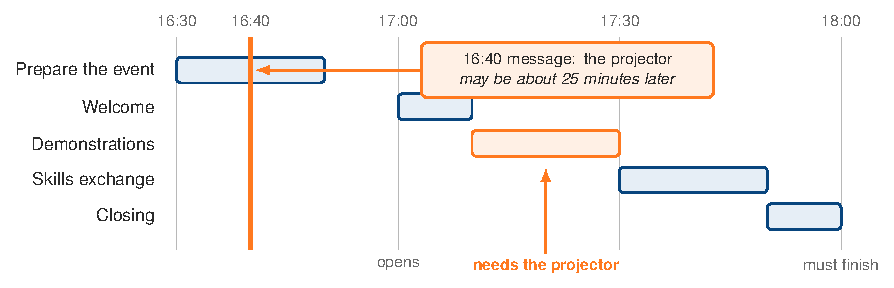
\includegraphics[width=0.86\textwidth]{fig_timeline.pdf}
  \end{center}
  \note{
    \textbf{(27s, ends 0:37)} Imagine you organize a campus showcase. It opens at five and
    must end by six. At four forty, a message says the projector may be twenty five minutes
    late. Change too much and people lose time. Wait too long and the demos fail. AI agents
    now act on messages like this. Would you wait, check, or prepare a backup?
  }
\end{frame}

% ~~~~~~~~~~~~~~~~~~~~~~~~~~~~~~~~~~~~~~~~~~~~~~~~~~~~~~~~~~~~~~~~~~~~~~~~~~~~~~
% 3. AUTHORITY (30 s)
\begin{frame}{The coordinator may check, hold and make free changes, not spend}
  \begin{itemize}
    \item Plan B is a \textbf{coordinator}: an AI agent with written limits.
    \item A \textbf{hold} is a free reservation of a backup that expires on its own, here worth up to \emphasize{\$35}.
    \item \textbf{Spending needs the organizer.} Participants and staff have their own narrow rights.
    \item Everything runs in a \textbf{fictional local sandbox}: no real bookings, purchases or messages.
  \end{itemize}
  \vspace{0.1cm}
  \begin{center}
    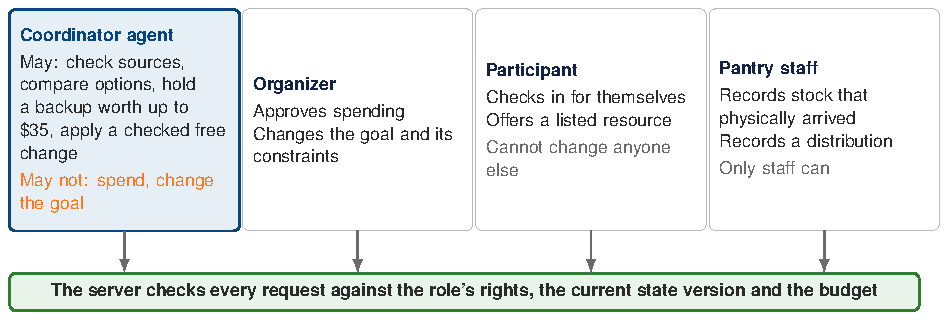
\includegraphics[width=0.97\textwidth]{fig_roles.pdf}
  \end{center}
  \note{
    \textbf{(30s, ends 1:07)} Plan B is a coordinator, an AI agent with written limits. It
    may check sources, compare options, place a hold, and make a change that costs nothing.
    A hold is a free reservation of a backup that expires on its own, here worth up to
    thirty five dollars. It cannot spend a cent without the organizer. Everything runs in a
    fictional local sandbox.
  }
\end{frame}

% ~~~~~~~~~~~~~~~~~~~~~~~~~~~~~~~~~~~~~~~~~~~~~~~~~~~~~~~~~~~~~~~~~~~~~~~~~~~~~~
% 4. VERIFY (31 s)
\begin{frame}{A message is a claim, not a fact}
  \begin{itemize}
    \item A \textbf{status check} asks the supplier's status service. It takes \emphasize{two simulated minutes} and returns a report, \textbf{not an arrival}.
  \end{itemize}
  \vspace{0.05cm}
  \begin{center}
    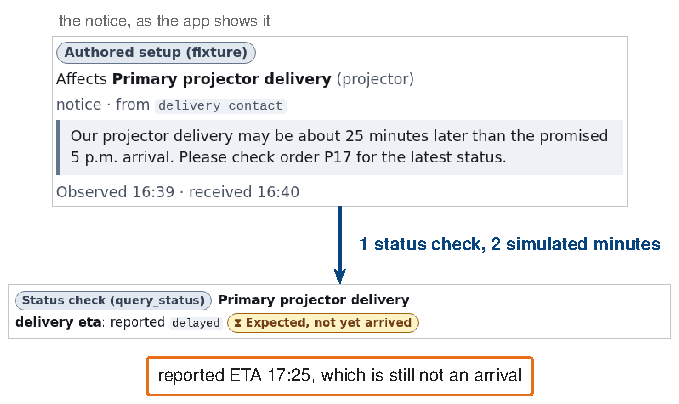
\includegraphics[height=7.3cm]{fig_claim.pdf}\\[2pt]
    \figcaption{Crops of the real app, from an automated run of development case dev01.}
  \end{center}
  \note{
    \textbf{(31s, ends 1:38)} Here is the notice, from the delivery contact. Plan B treats
    it as a claim, not a fact. Before changing anything, it checks the one fact that could
    change the decision. A status check asks the supplier's status service. The answer is
    delayed, with a reported arrival at five twenty five. Even that is a report, not an
    arrival, so the plan must still work if it slips.
  }
\end{frame}

% ~~~~~~~~~~~~~~~~~~~~~~~~~~~~~~~~~~~~~~~~~~~~~~~~~~~~~~~~~~~~~~~~~~~~~~~~~~~~~~
% 5. COMMIT (44 s)
\begin{frame}{One checked change, one receipt}
  \begin{itemize}
    \item The \textbf{planner} builds the allowed repairs and checks each: \emphasize{16 built, 3 pass}. Best: a swap that \emphasize{costs \$0}.
    \item A \textbf{receipt} is the server's own record of an accepted change. The AI cannot write it.
  \end{itemize}
  \vspace{0.05cm}
  \begin{center}
    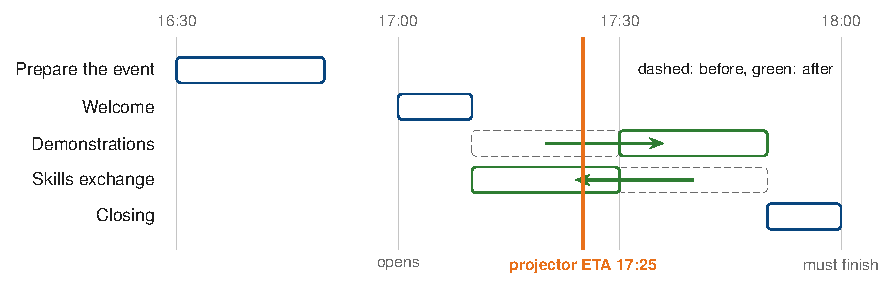
\includegraphics[width=0.84\textwidth]{fig_swap.pdf}\\[4pt]
    \fcolorbox{muted}{white}{
\includegraphics[width=0.84\textwidth]{receipt_line.png}}\\[3pt]
    \figcaption{Shown: my fixed-rule baseline in an automated run. In a recorded practice run, the AI coordinator made the same check and the same swap at 16:43.}
  \end{center}
  \note{
    \textbf{(44s, ends 2:22)} The planner builds the allowed repairs from fixed templates
    and checks each against the deadline, the people, and the budget. Sixteen are built and
    three pass. The best is free: swap the demonstrations with the skills exchange, so the
    demos start at five thirty, after the reported arrival. It is applied at four forty
    three, and the server writes a receipt, its own record of the change. The AI cannot
    write it. These frames show my rule baseline. In a recorded run, the AI coordinator made
    the same check and the same swap.
  }
\end{frame}

% ~~~~~~~~~~~~~~~~~~~~~~~~~~~~~~~~~~~~~~~~~~~~~~~~~~~~~~~~~~~~~~~~~~~~~~~~~~~~~~
% 6. KEEP (47 s)
\begin{frame}{Four messages, zero changes}
  \begin{itemize}
    \item A second practice case, \textbf{in the order it happened}.
    \item Not acting is the harder skill: \emphasize{no hold, no spending, no change}.
  \end{itemize}
  \vspace{0.15cm}
  \begin{center}
    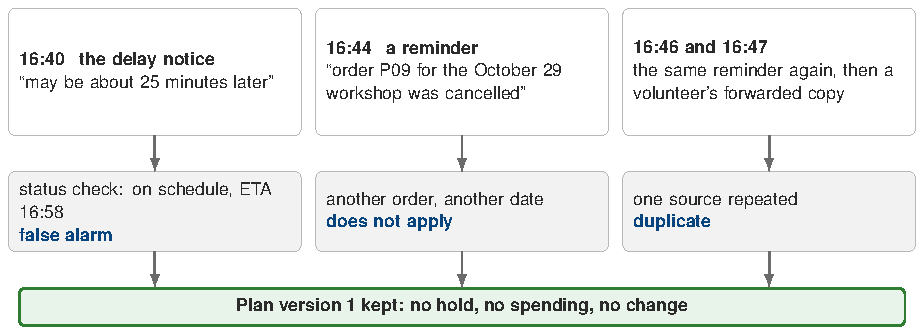
\includegraphics[width=0.95\textwidth]{fig_quiet.pdf}\\[3pt]
    \figcaption{Development case dev04, decided by the rule baseline in an automated run of the app.}
  \end{center}
  \note{
    \textbf{(47s, ends 3:09)} Not acting is the harder skill. Here is a second practice
    case. First, the same delay notice, but the status check says on schedule, arriving at
    four fifty eight. A false alarm, so the plan stays. Then a reminder that order P nine
    for an October workshop was cancelled. That is another order on another date, so it does
    not apply. [Skip if late: It arrives again, and a volunteer forwards it. One source
    repeated is still one source.] In the end there is no hold, no spending and no change.
    Three of my twelve final test cases are quiet ones like this.
  }
\end{frame}

% ~~~~~~~~~~~~~~~~~~~~~~~~~~~~~~~~~~~~~~~~~~~~~~~~~~~~~~~~~~~~~~~~~~~~~~~~~~~~~~
% 7. THE LOOP (26 s)
\begin{frame}{Verify, prepare, commit}
  \vspace{-0.1cm}
  \begin{center}
    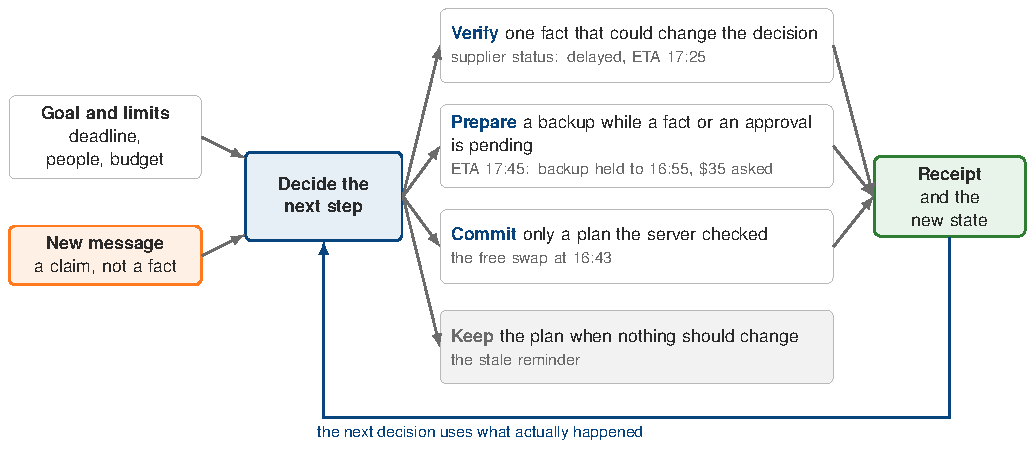
\includegraphics[width=\textwidth]{fig_loop.pdf}
  \end{center}
  \vspace{-0.1cm}
  \begin{itemize}
    \item \textbf{Prepare} example: the projector arrives too late, so the backup is \emphasize{held until 16:55} while the organizer decides on \$35.
  \end{itemize}
  \note{
    \textbf{(26s, ends 3:35)} Verify one fact that could change the decision. Prepare a
    backup while a fact or an approval is pending. In another case the projector arrives too
    late, so Plan B holds the backup until four fifty five and asks the organizer for thirty
    five dollars. Commit only a plan the server checked. Or keep the plan.
  }
\end{frame}

% ~~~~~~~~~~~~~~~~~~~~~~~~~~~~~~~~~~~~~~~~~~~~~~~~~~~~~~~~~~~~~~~~~~~~~~~~~~~~~~
% 8. THE MODEL CHOOSES, THE SERVER CHECKS (30 s)
\begin{frame}{The model chooses, the server checks}
  \begin{itemize}
    \item A \textbf{policy} is the rule that picks the next step. Rules read only the messages they were written for. A \textbf{model} reads any wording, so it chooses and \emphasize{the server checks}.
  \end{itemize}
  \vspace{0.05cm}
  \begin{center}
    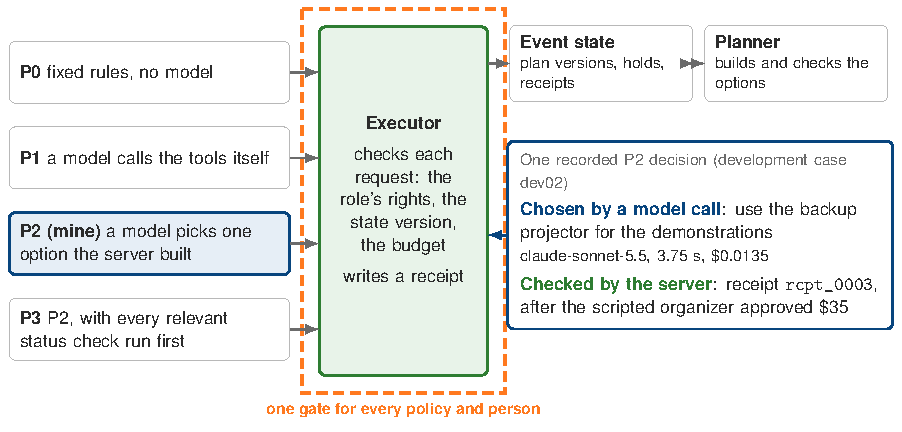
\includegraphics[width=0.9\textwidth]{fig_architecture.pdf}
  \end{center}
  \note{
    \textbf{(30s, ends 4:05)} A policy is the rule that picks the next step. P zero is fixed
    rules, which only read the messages they were written for. P one lets a model call the
    tools freely. P two, mine, lets the model pick from options the server built and
    checked. P three is P two with every relevant check run first. Every policy passes the
    same gate.
  }
\end{frame}

% ~~~~~~~~~~~~~~~~~~~~~~~~~~~~~~~~~~~~~~~~~~~~~~~~~~~~~~~~~~~~~~~~~~~~~~~~~~~~~~
% 9. THE HELD-OUT TEST, VERSION 1.1 (38 s)
\begin{frame}{Held-out test of version 1.1: zero violations, no clear winner}
  \begin{itemize}
    \item \textbf{Held-out cases}: locked before the test and hidden from every policy. Code, prompts, model and limits were \textbf{frozen} first. A run is \textbf{met} when its final state and receipts show the case's outcome.
  \end{itemize}
  \begin{center}
    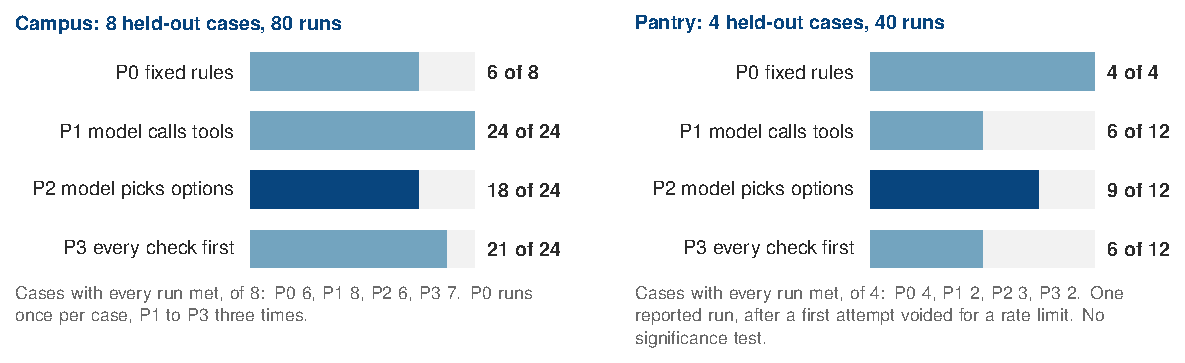
\includegraphics[width=\textwidth]{fig_results.pdf}
  \end{center}
  \vspace{-0.1cm}
  \begin{itemize}
    \item All \res{both:recorded} runs recorded. Every policy: \textbf{\res{both:viol} executed violations}, \textbf{\res{both:unnec} changes} on the 3 quiet cases. Refused: \res{campus:all:refused} campus and \res{pantry:all:refused} pantry requests (\res{both:stale} on a state that changed meanwhile).
    \item \emphasize{No consistent advantage for P2.} Campus model cost: P1 met \res{campus:P1:metk} of \res{campus:P1:metn} runs for \$\res{campus:P1:usd}, P3 \res{campus:P3:metk} for \$\res{campus:P3:usd}, P2 \res{campus:P2:metk} for \$\res{campus:P2:usd}. Fixed rules met every pantry run.
  \end{itemize}
  \note{
    \textbf{(38s, ends 4:43)} Everything so far came from practice cases I built with. Then
    I froze version one point one, its code, prompts, model and limits, and ran twelve
    held-out cases, hidden from every policy. All one hundred twenty runs were recorded. No
    policy executed a violation or changed a quiet event. But my P two showed no consistent
    advantage. P one met the expected outcome in all twenty four campus runs, at three times
    P two's model cost. These are descriptive counts only.
  }
\end{frame}

% ~~~~~~~~~~~~~~~~~~~~~~~~~~~~~~~~~~~~~~~~~~~~~~~~~~~~~~~~~~~~~~~~~~~~~~~~~~~~~~
% 10. ONE FAILURE (26 s)
\begin{frame}{One failure: a correct reading that never reached the planner}
  \begin{itemize}
    \item Held-out case \textbf{C06}: a volunteer will be late, with a later check-in.
    \item P2 and P3 failed it in all \textbf{6 runs}, and every one stays \textbf{in the count}. P1 met it in 3 of 3.
  \end{itemize}
  \vspace{0.25cm}
  \begin{center}
    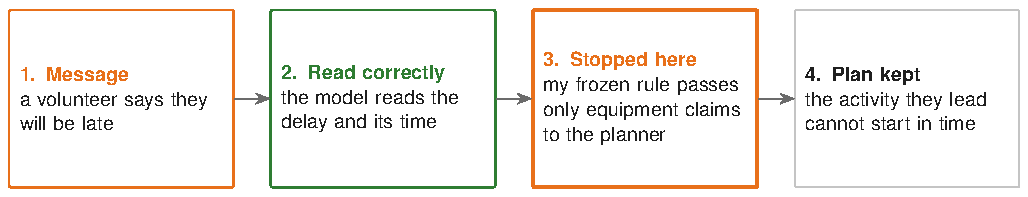
\includegraphics[width=\textwidth]{fig_failure.pdf}\\[6pt]
    \figcaption{From the run's failure analysis. Other failures: the limit of 8 model calls per run ended 15 of the 26 failed runs (backup).}
  \end{center}
  \vspace{0.2cm}
  \begin{itemize}
    \item The reading was right. My frozen rule dropped it before the planner (the \textbf{planner input} stage), a limit disclosed before the runs.
  \end{itemize}
  \note{
    \textbf{(26s, ends 5:09)} In one held-out case a volunteer says they will be late. P two
    and P three read the message correctly. But my frozen rule passes only equipment claims
    to the planner, so the plan was never questioned. All six of their runs stay in the
    count. P one met this case every time.
  }
\end{frame}

% ~~~~~~~~~~~~~~~~~~~~~~~~~~~~~~~~~~~~~~~~~~~~~~~~~~~~~~~~~~~~~~~~~~~~~~~~~~~~~~
% 11. PANTRY (40 s)
\begin{frame}{Same loop, a new rule: 40 kits for a fictional pantry}
  \begin{itemize}
    \item Staff need \textbf{40 kits by 13:40}. 24 are on the shelf, \emphasize{20 are late and do not count}, 16 wait in a partner pool.
    \item Only \textbf{staff} record the handoff and the distribution. The agent can hold kits but never records them.
  \end{itemize}
  \vspace{0.05cm}
  \begin{center}
    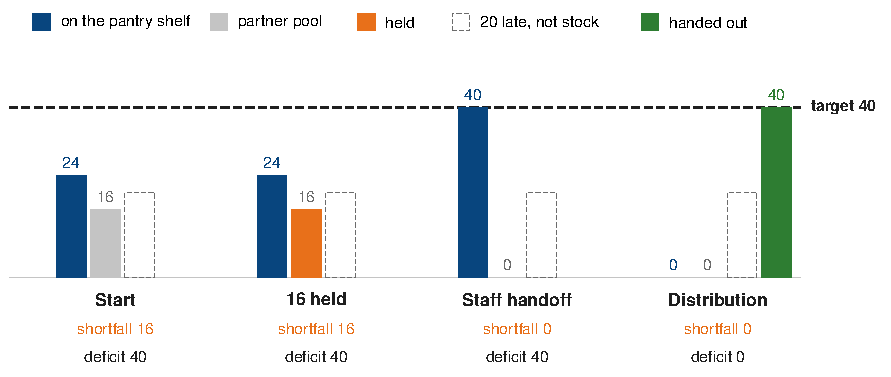
\includegraphics[width=0.74\textwidth]{fig_pantry.pdf}\\[2pt]
    \figcaption{\textbf{Shortfall}: kits still missing from the shelf. \textbf{Deficit}: kits not yet handed out. Fictional pantry sandbox, development case pantry\_dev01.}
  \end{center}
  \vspace{-0.1cm}
  \begin{itemize}
    \item \textbf{Held-out pantry, version 1.1}: rules met \res{pantry:P0:metk} of \res{pantry:P0:metn} runs, model policies \res{pantry:P1:metk} to \res{pantry:P2:metk} of 12, partly from a frozen planner defect (T03). \emphasize{No kit counted twice.}
  \end{itemize}
  \note{
    \textbf{(40s, ends 5:49)} The same loop runs a fictional pantry. Staff need forty kits
    by one forty. Twenty four are on the shelf. Twenty more are late, and late stock does
    not count. Sixteen wait in a partner pool. Plan B holds those sixteen. Only staff record
    the handoff and the distribution. On four held-out pantry cases, fixed rules met all
    four runs, and the model policies six to nine of twelve, partly because of a defect in
    my frozen planner. No kit was counted twice.
  }
\end{frame}

% ~~~~~~~~~~~~~~~~~~~~~~~~~~~~~~~~~~~~~~~~~~~~~~~~~~~~~~~~~~~~~~~~~~~~~~~~~~~~~~
% 12. VERSION 1.2 (39 s)
\begin{frame}{Version 1.2: the fixes, then six fresh held-out cases}
  \begin{itemize}
    \item \textbf{Fixed after the held-out failures}: a person's own delay now reaches the planner (C06), a pool checked as unavailable is no longer offered (T03), a menu the model declined is not sent again, and a rate limit is waited out.
    \item \textbf{Fresh held-out set}: 6 new cases, C09 to C12, T05 and T06, written without the new code and \textbf{locked before the first 1.2 call}. Same model and limits.
  \end{itemize}
  \vspace{0.1cm}
  \begin{center}
  {\small
  \setlength{\tabcolsep}{4pt}
  \begin{tabular}{@{}lcccc@{\hspace{12pt}}cccc@{}}
    \toprule
    & \multicolumn{4}{c}{\textbf{Campus runs met}} & \multicolumn{4}{c}{\textbf{Pantry runs met}} \\
    & P0 & P1 & P2 & P3 & P0 & P1 & P2 & P3 \\
    \midrule
    Version 1.1: 12 cases, the record & \res{campus:P0:met} & \res{campus:P1:met} & \res{campus:P2:met} & \res{campus:P3:met} & \res{pantry:P0:met} & \res{pantry:P1:met} & \res{pantry:P2:met} & \res{pantry:P3:met} \\
    Version 1.2: 6 different, fresh cases & \res{fresh:campus:P0:met} & \res{fresh:campus:P1:met} & \res{fresh:campus:P2:met} & \res{fresh:campus:P3:met} & \res{fresh:pantry:P0:met} & \res{fresh:pantry:P1:met} & \res{fresh:pantry:P2:met} & \res{fresh:pantry:P3:met} \\
    \bottomrule
  \end{tabular}\par}
  \end{center}
  \vspace{0.05cm}
  \begin{itemize}
    \item \emphasize{\res{fresh:both:metk} of \res{fresh:both:metn} fresh runs met}, \res{fresh:both:viol} executed violations. The miss: P0 on C11, a person's own delay that its rules cannot read. P1 to P3 met every run, so this small set \textbf{cannot rank them}.
  \end{itemize}
  \vspace{0.05cm}
  \figcaption{Different cases, so the two rows are not a before and after. The fresh cases repeat known conditions (C11 is the C06 condition, T06 is T03). Descriptive counts, no significance test. A post-hoc rerun of 1.2 on the spent cases is diagnostic only, not held-out (backup).}
  \note{
    \textbf{(39s, ends 6:28)} Version one point two targets those failures. A person's own
    delay now reaches the planner, and a pool checked as unavailable is no longer offered.
    The old cases were spent, so six fresh ones were written without the new code, and
    locked before any call. Version one point two met fifty nine of sixty runs. Fixed rules
    missed one late volunteer. The other policies met every run, so this small set cannot
    rank them. The cases differ, so this is not a before and after.
  }
\end{frame}

% ~~~~~~~~~~~~~~~~~~~~~~~~~~~~~~~~~~~~~~~~~~~~~~~~~~~~~~~~~~~~~~~~~~~~~~~~~~~~~~
% 13. CLOSE (32 s)
\begin{frame}{What works today, and what is next}
  \begin{columns}[T,onlytextwidth]
    \column{0.7\textwidth}
      \begin{itemize}
        \item \textbf{Works}: verify, prepare, commit in a local sandbox. Every accepted change has a \emphasize{receipt}, and people approve spending.
        \item \textbf{Tested} on 12 held-out cases (\res{both:recorded} runs), then version 1.2 on 6 fresh ones (\res{fresh:both:recorded} runs): \emphasize{zero executed violations}, and no clear winner among the policies.
        \item \textbf{In real life} a message is a text, a status check is a tracking page, a hold is a refundable reservation.
        \item \textbf{Not shown}: real bookings, real stock, a community pilot. \textbf{Next}: review the workflows with community staff.
      \end{itemize}
    \column{0.28\textwidth}
      \centering
      
\includegraphics[width=1.0\textwidth]{fig_qr.pdf}\\[2pt]
      {\footnotesize github.com/nocdoggo/COLLIE\\ branch hackathon/peeaai-plan\\ app in apps/plan\_b\par}
  \end{columns}
  \vfill
  \begin{columns}[c,onlytextwidth]
    \column{0.7\textwidth}
      \textbf{Noctis Zhang}\\
      University of Massachusetts Boston
    \column{0.3\textwidth}
      \hfill
\includegraphics[height=1.0cm]{Blue-UMB-logo-lockup.png}
  \end{columns}
  \note{
    \textbf{(32s, ends 7:00)} Today Plan B verifies, prepares and commits in a local
    sandbox. Every accepted change has a receipt, and people approve spending. In both
    held-out tests no policy executed a violation, and my policy showed no consistent
    advantage. In real life a message is a text, a status check is a tracking page, and a
    hold is a refundable reservation. No community has used it yet. Next, I want to review
    it with community staff. Thank you.
  }
\end{frame}

% ~~~~~~~~~~~~~~~~~~~~~~~~~~~~~~~~~~~~~~~~~~~~~~~~~~~~~~~~~~~~~~~~~~~~~~~~~~~~~~
% BACKUP SLIDES (not timed)
\appendix
\begin{frame}{Backup: one model decision, as recorded}
  \begin{columns}[T,onlytextwidth]
    \column{0.42\textwidth}
      \begin{itemize}
        \item A \textbf{replay} re-shows a recorded run. It never calls a tool and is never a new trial.
        \item A development run of P2 on case dev02, recorded with an earlier version (\texttt{live/1.0.0}) before the freeze.
        \item The model chose one option the server built. The server checked it and wrote the receipt. The model's own rationale is shown as \emphasize{untrusted text}.
      \end{itemize}
    \column{0.56\textwidth}
      \centering
      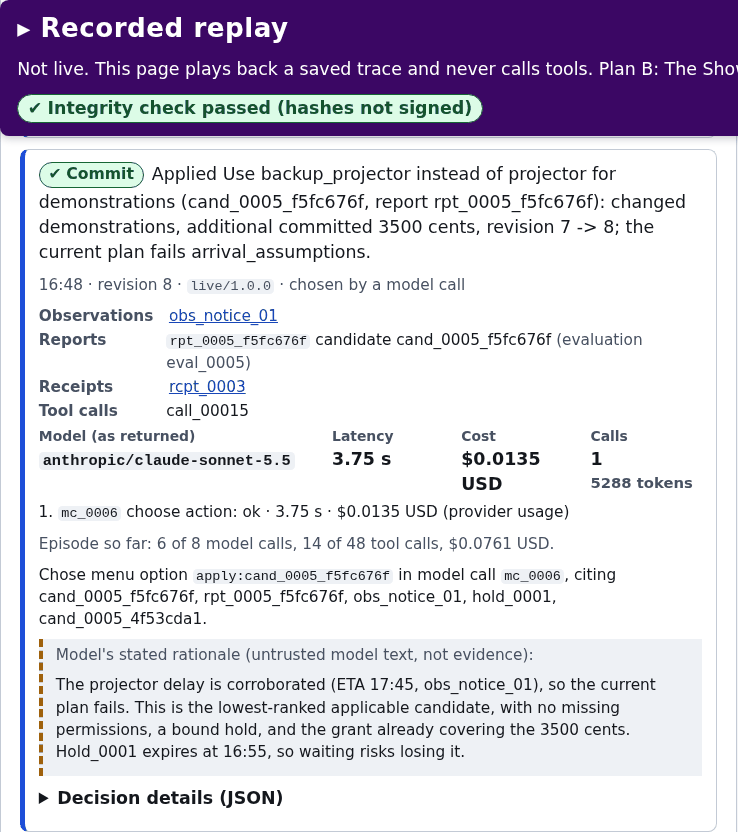
\includegraphics[height=8.1cm]{live_card.png}
  \end{columns}
\end{frame}

\begin{frame}{Backup: the report's per-case figure, campus}
  \begin{center}
    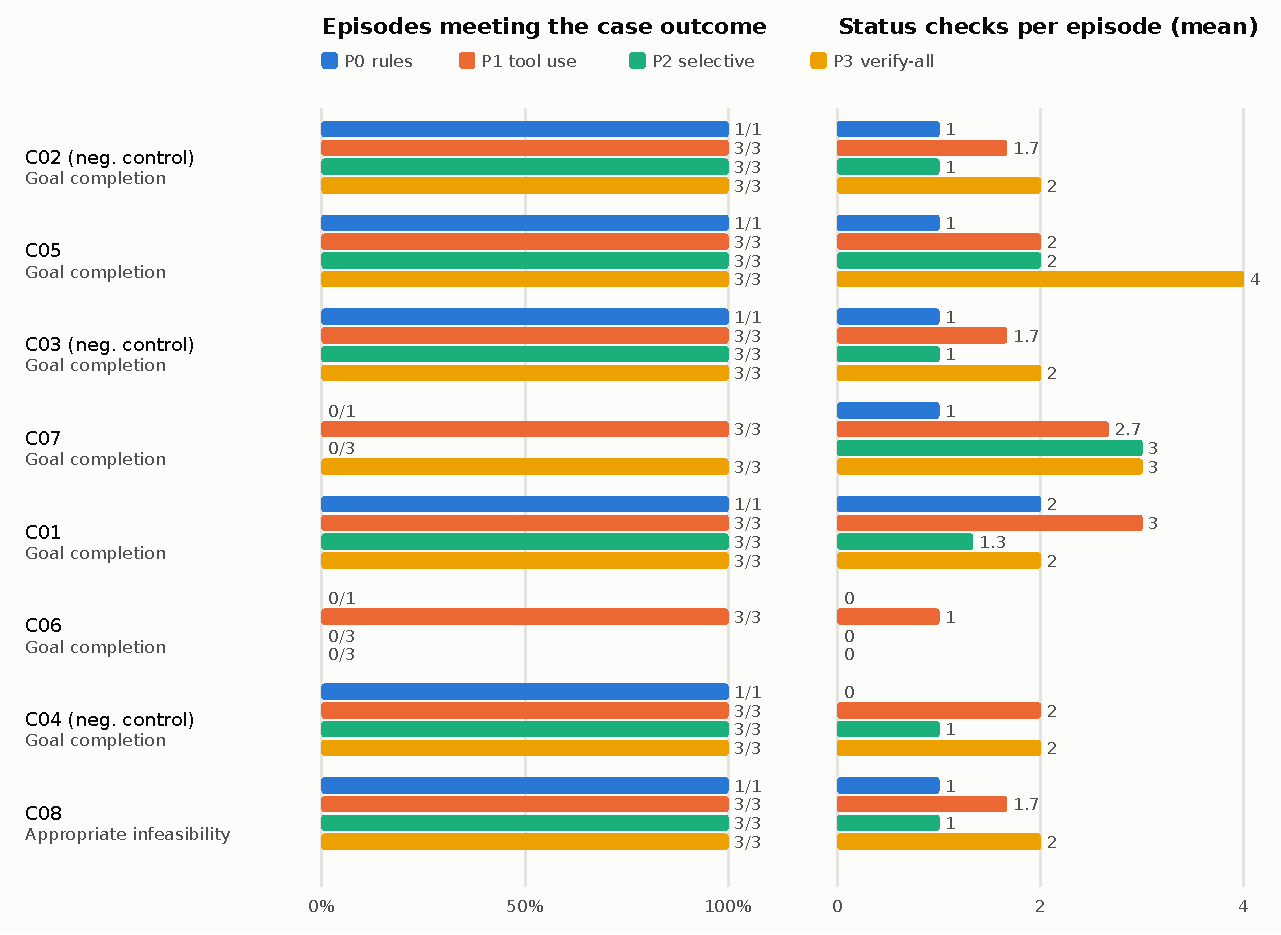
\includegraphics[height=8.2cm]{report_campus.pdf}\\[2pt]
    \figcaption{\texttt{campus/report/figure.svg} of run wave3\_heldout\_20261025T1625Z, printed to PDF. Case order as in the report. Legend: P1 tool use is P1 model calls tools, P2 selective is P2 model picks options, P3 verify-all is P3 every check first.}
  \end{center}
\end{frame}

\begin{frame}{Backup: the report's per-case figure, pantry}
  \begin{center}
    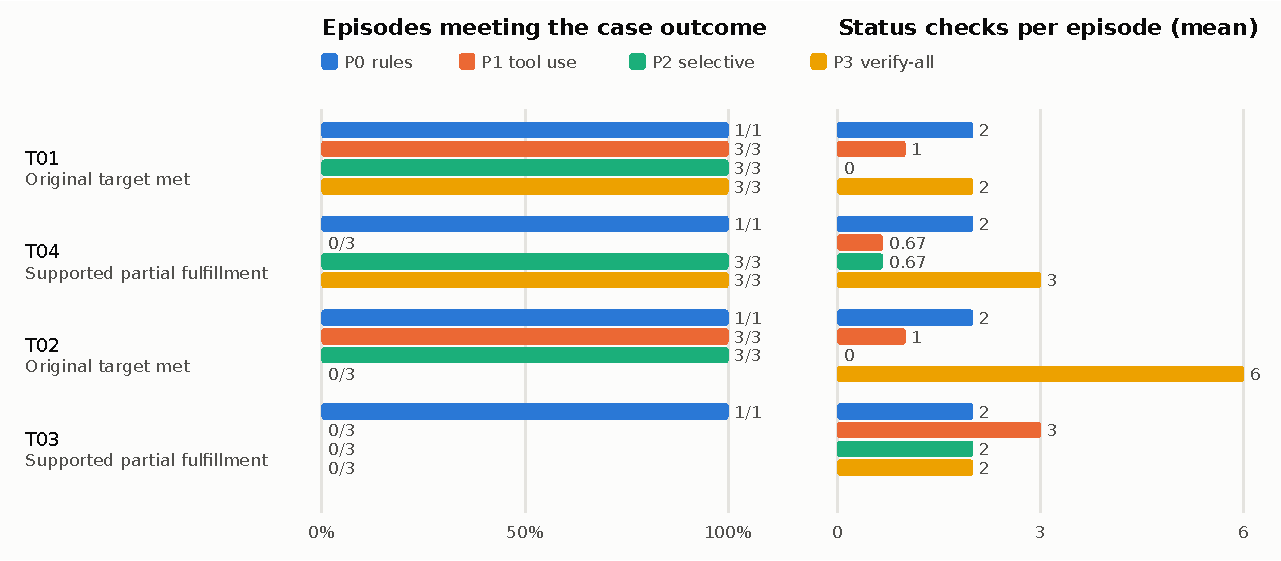
\includegraphics[width=0.92\textwidth]{report_pantry.pdf}\\[2pt]
    \figcaption{\texttt{pantry/report/figure.svg} of the same run, printed to PDF. Case order as in the report.}
  \end{center}
\end{frame}

\begin{frame}{Backup: what the held-out runs cost}
  \begin{center}
  {\small
  \setlength{\tabcolsep}{6pt}
  \begin{tabular}{@{}lcccc@{}}
    \toprule
    & \multicolumn{2}{c}{\textbf{Campus}} & \multicolumn{2}{c}{\textbf{Pantry}} \\
    \textbf{Policy} & \textbf{Model calls} & \textbf{Model USD} & \textbf{Model calls} & \textbf{Model USD} \\
    \midrule
    P0 fixed rules & \res{campus:P0:calls} & \res{campus:P0:usd} & \res{pantry:P0:calls} & \res{pantry:P0:usd} \\
    P1 model calls tools & \res{campus:P1:calls} & \res{campus:P1:usd} & \res{pantry:P1:calls} & \res{pantry:P1:usd} \\
    P2 model picks options & \res{campus:P2:calls} & \res{campus:P2:usd} & \res{pantry:P2:calls} & \res{pantry:P2:usd} \\
    P3 every check first & \res{campus:P3:calls} & \res{campus:P3:usd} & \res{pantry:P3:calls} & \res{pantry:P3:usd} \\
    \bottomrule
  \end{tabular}\par}
  \end{center}
  \begin{itemize}
    \item Provider-reported cost of the reported run of version 1.1. Version 1.2 cost \$\res{fresh:both:usd} for the \res{fresh:both:recorded} fresh held-out runs and \$\res{rerun:both:usd} for the \res{rerun:both:recorded} runs of the diagnostic rerun. Runs of 1.1 stopped by the 8-call limit: campus \res{campus:all:capped}, pantry \res{pantry:all:capped}, so \res{both:capped} runs, 15 of them among the 26 failed runs. All stay in the counts.
    \item A first attempt was \textbf{voided} before the reported run began: the provider's rate limit (20 requests a minute) answered most calls with an error. It is kept on record. The frozen status rules would have scored its capped runs, so the void is a disclosed departure from them. The whole protocol was rerun one run at a time.
  \end{itemize}
\end{frame}

\begin{frame}{Backup: what the held-out numbers do not show}
  \begin{itemize}
    \item \textbf{The case is the unit}: 8 campus and 4 pantry cases. Three runs of a case are repeated trials. No significance test.
    \item \textbf{C06} is out of reach for P0, P2 and P3 by a frozen rule, disclosed before the runs.
    \item \textbf{Pantry}: only P2 and P3 had pantry guidance in their prompts. A defect in my frozen planner kept a pool checked as unavailable on offer, and it is where each of the six P2 and P3 failures on case T03 first went wrong.
    \item The 8 model calls per run come from development and ended 15 of the 26 failed runs.
    \item These 12 cases are now spent. Version 1.2 got 6 new cases and a new freeze.
    \item \textbf{Version 1.2}: 6 cases are few, and they repeat known conditions with near copies of the old wording. Five limits found by the audit before the freeze stay frozen, so that no one who had seen the new cases changed a policy.
  \end{itemize}
\end{frame}

\begin{frame}{Backup: version 1.2 on the spent cases, a diagnostic rerun}
  \begin{itemize}
    \item \textbf{Post-hoc diagnostic rerun after fixes, on spent cases. Not a held-out result.} The fixes were made after reading these failures.
  \end{itemize}
  \vspace{0.1cm}
  \begin{center}
  {\small
  \setlength{\tabcolsep}{4pt}
  \begin{tabular}{@{}lcccc@{\hspace{12pt}}cccc@{}}
    \toprule
    & \multicolumn{4}{c}{\textbf{Campus runs met}} & \multicolumn{4}{c}{\textbf{Pantry runs met}} \\
    & P0 & P1 & P2 & P3 & P0 & P1 & P2 & P3 \\
    \midrule
    Version 1.1, held-out record & \res{campus:P0:met} & \res{campus:P1:met} & \res{campus:P2:met} & \res{campus:P3:met} & \res{pantry:P0:met} & \res{pantry:P1:met} & \res{pantry:P2:met} & \res{pantry:P3:met} \\
    Version 1.2, diagnostic rerun & \res{rerun:campus:P0:met} & \res{rerun:campus:P1:met} & \res{rerun:campus:P2:met} & \res{rerun:campus:P3:met} & \res{rerun:pantry:P0:met} & \res{rerun:pantry:P1:met} & \res{rerun:pantry:P2:met} & \res{rerun:pantry:P3:met} \\
    \bottomrule
  \end{tabular}\par}
  \end{center}
  \vspace{0.05cm}
  \begin{itemize}
    \item Consistent with the fixes: P1 to P3 met every run on C06 and T03. Still failing, as in 1.1: C07 under P2 (the call budget spent on hold churn), T02 under P3 (a stale apply), T04 under P1 in 2 of 3 runs, and P0 on C06 and C07.
    \item Run two at a time: \res{rerun:both:capped} runs stopped at the 8-call limit, and 61 rate-limit answers were waited out at no cost. \res{rerun:both:viol} executed violations.
  \end{itemize}
\end{frame}

\begin{frame}{Backup: a development failure, kept on record}
  \begin{itemize}
    \item In development, P1's first run on the pantry practice case: the executor \textbf{refused 6 holds}, the model call limit was reached, \emphasize{0 of 40} kits were served.
    \item Cause: a defect in my P1 harness. The prompt never said which time window a hold covers, and the reply limit counted the model's reasoning.
    \item Fixed in the prompt and the limit. The rerun served \emphasize{40 of 40}. The failed run is kept.
  \end{itemize}
\end{frame}

\begin{frame}{Backup: a participant's own check-in changes the plan}
  \begin{center}
    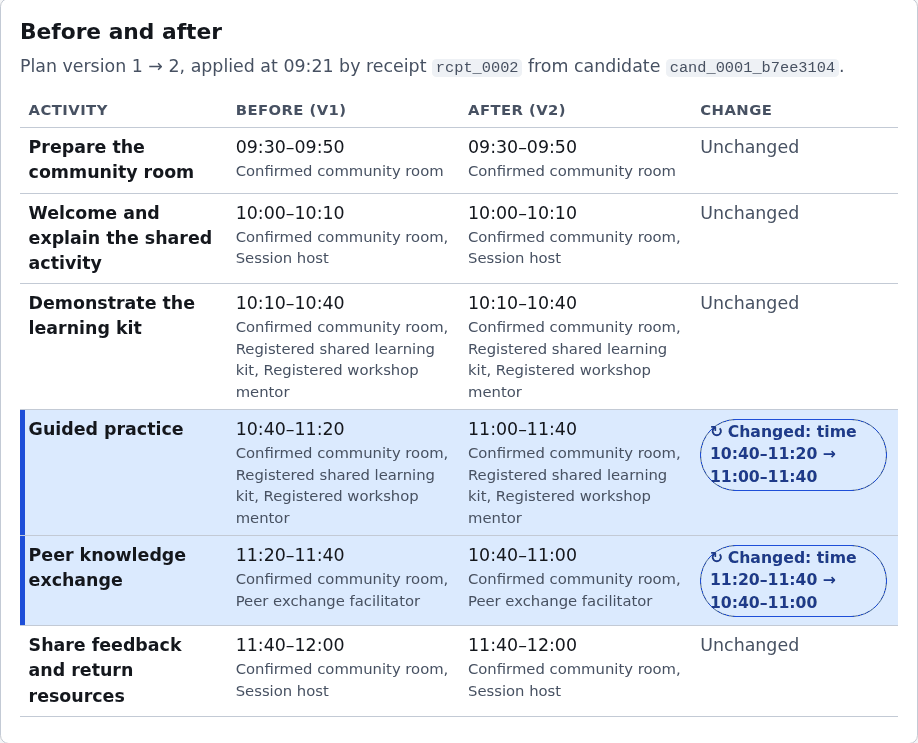
\includegraphics[height=7.6cm]{community_replanned.png}\\[3pt]
    \figcaption{Development case skills\_dev01: the peer lead can stay only until 11:05, so the plan swaps two activities. P0 fixed rules, automated run.}
  \end{center}
\end{frame}

\begin{frame}{Backup: a partial handoff stays partial}
  \begin{itemize}
    \item Development case pantry\_dev02: staff hand off only \textbf{10 of the 16} kits.
    \item \emphasize{34 kits} are distributed and a \emphasize{6-kit deficit} is reported. The target stays 40.
    \item Stock is conserved: 34 handed out plus 6 left in the partner pool make 40. The 20 kits of the late shipment never count as stock.
  \end{itemize}
\end{frame}

\begin{frame}{Backup: the frozen configurations}
  \begin{itemize}
    \item \textbf{Policies}: P0 \texttt{rules/1.0.0} and \texttt{pantry-rules/1.1.0}, P1 \texttt{tool-use/1.1.0}, P2 \texttt{live/1.1.0}, P3 \texttt{verify-all/1.1.0}.
    \item \textbf{Model}: \texttt{anthropic/claude-sonnet-5.5} through OpenRouter, the same for P1 to P3.
    \item \textbf{Limits per run}: 48 tool calls, 8 model calls, \$0.50, 900 seconds.
    \item \textbf{Seeds} 101, 202 and 303 are recorded but not sent, because the model's endpoints refuse a seed. The three runs of a case are repeated trials, not reproducible ones.
    \item Frozen by hash in \texttt{freeze.json} before the first held-out call.
    \item \textbf{Version 1.2}: P1 \texttt{tool-use/1.2.0}, P2 \texttt{live/1.2.0}, P3 \texttt{verify-all/1.2.0}, P0 unchanged on planner 1.2.0. Same model and limits. Frozen in \texttt{freeze\_v1\_2.json} at 23:23:47 UTC, the fresh cases locked at 23:23:54, the first call at 23:27:31.
  \end{itemize}
\end{frame}

\end{document}
